%=========================================================
\chapter{Modelo dinámico}

%---------------------------------------------------------
\section{Modelo de casos de uso}

	En la figura~\ref{fig:casosdeuso} se muestra el diagrama de casos de uso.

\begin{figure}[htbp!]
	\centering
		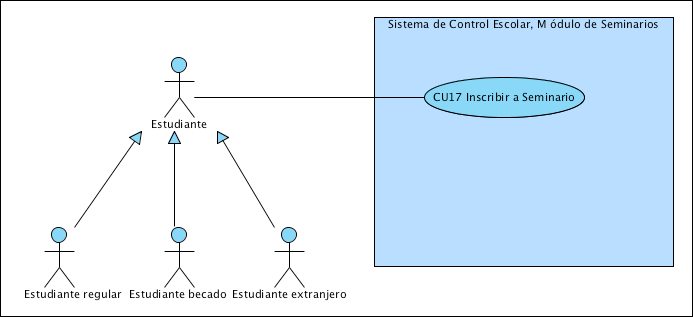
\includegraphics[width=0.8\textwidth]{images/CasosDeUso}
	\caption{Diagrama de Casos de Uso del sistema.}
	\label{fig:casosdeuso}
\end{figure}

%---------------------------------------------------------
\cfinput{actores}

%---------------------------------------------------------
\section{Especificación de casos de uso}

	En este capítulo se describen cada uno de los casos de uso del sistema. De cada caso de uso se detallan los siguientes elementos:\\
	
\begin{Citemize}
	\item {\bf Resumen:} Describe brevemente las condiciones que dan pie al caso de uso, la operación que se realiza y las consecuencias de ejecutarlo.
%	\item {\bf Herencia:} Indica si el caso de uso es una forma particular de otro y de ser así, indica de cuál.
	\item {\bf Actores:} Enlista a los usuarios que intervienen en el caso de uso.
	\item {\bf Propósito:} Indica la razón por la que se ejecuta el caso de uso.
	\item {\bf Entradas:} Detalla la información que debe ser ingresada al sistema para la ejecución del caso de uso.
	\item {\bf Salidas:} Enlista toda la información y resultados que son mostrados por el sistema.
	\item {\bf Origenes:} Detalla los orígenes de los datos de entrada.
	\item {\bf Destinos:} Detalla los destinos de los datos de salida.
	\item {\bf Precondiciones:} Indica los requisitos para que el caso de uso pueda ser ejecutado.
	\item {\bf Postcondiciones:} Describe las consecuencias y el impacto que genera el ejecutar exitosamente el caso de uso.
	\item {\bf Errores:} Enlista los casos en que no se podrá terminar el caso de uso de manera adecuada.
	% \item {\bf Tipo:} Indica si el caso de uso puede ser accesado directamente o se desprende de otro.
	\item {\bf Fuente:} Especifica el origen principal de información empleada para la elaboración del caso de uso.
	\item {\bf Observaciones:} Presenta información o comentarios dirigidos a las personas que lean el caso de uso.
	\item {\bf Trayectorias:} Muestra el flujo de pasos que se siguen para la ejecución correcta del caso de uso, así como las variaciones que pueden presentarse durante su ejecución.
	\item {\bf Trayectorias alternativas:} Describe las variaciones que pueden presentarse durante la ejecución del caso de uso.
	\item {\bf Autor:} Nombre del analista responsable de especificar el caso de uso.
	\item {\bf Versión:} Numero con punto decimal que indica la versión del Caso de Uso.
	\item {\bf Modificado:} Fechas de modificación.
	\item {\bf Revisor:} Nombre del analista responsable de revisar el Caso de Uso.
	\item {\bf Revisado:} Fecha en que se realizó la última revisión (si aun no se revisa se deja en ``Pendiente por revisar'').
	\item {\bf Status:} Puede ser: Edición (el analista aun no termina de detallar o hay observaciones pendientes por parte del revisor), Revisado (El Revisor aprobó la descripción del caso de uso), Aprobado(El usuario aprueba la descripción del  Caso de uso).
	\item {\bf Aprobado:} Fecha en que se realizó la aprobación por parte del cliente (si aun no se aprobar se deja en ``Pendiente por aprobar'').
	\item {\bf Madurez:} Puede ser Alta, Media o Baja, dependiendo el grado en que el Caso de Uso es comprendido por el Analista, Revisor y Cliente.
	\item {\bf Volatilidad:} Puede ser Alta, Media o Baja, dependiendo la cantidad y magnitud de cambios que haya recibido el caso de uso, el numero de versiones existentes o probabilidad de que cambie en corto plazo.
	\item {\bf Dificultad:} Puede ser Alta, Media o Baja, dependiendo el esfuerzo que se requerirá para desarrollar y probar el Caso de Uso.
	\item {\bf Prioridad:} Puede ser Alta, Media o Baja, dependiendo el grado de importancia para el negocio, el cliente o el sponsor.
	%\item {\bf Puntos de extensión:} Indica los casos de uso que pueden desprenderse de su ejecución.
\end{Citemize}

\cfinput{cu17/cu}
